% ---------------------------------------------------------------
% ---------------------------------------------------------------
% This template was developed for the working paper series of 
% the Interdisciplinary Laboratory of Computational Social Science (iLCSS)
% at the University of Maryland, College Park

% The template was built based on  the PNAS Latex model. 

% Adjustments were made by Tiago Ventura, Ph.D. Candidate in Political Science at UMD, and researcher at the iLCSS.

\documentclass[9pt,twocolumn,twoside]{ilcss}
\usepackage{amsthm}
\usepackage{amsmath}
\usepackage{algorithm}
\usepackage[noend]{algpseudocode}
\usepackage[dvipsnames]{xcolor}

\theoremstyle{definition}
\newtheorem{definition}{Definition}[section]

\theoremstyle{remark}
\newtheorem{remark}{Remark}[section]

\theoremstyle{definition}
\newtheorem*{goal}{Goal}

\theoremstyle{definition}
\newtheorem*{hypothesis}{Hypothesis}

\templatetype{ilcssworkingpaper} % Choose template 

\title{AI Models and Applications report: Face Recognition}	

% Use letters for affiliations, numbers to show equal authorship (if applicable) and to indicate the corresponding author
\author[a]{Arno Lesage (no. 22202985)}
\author[a]{Minh Quan Hoang  (no. hm509118)}

\affil[a]{Université Côte d'Azur EUR - DS4H - Master 1 Informatique, parcours IA}
% Please include corresponding author, author contribution and author declaration information
\authordeclaration{Used \LaTeX{} templates: iLCSS Working Paper Template by Ernesto Calvo et Tiago Ventura under Creative Commons CC BY 4.0.}
%\equalauthors{}

% Keywords are not mandatory, but authors are strongly encouraged to provide them. If provided, please include two to five keywords, separated by the pipe symbol, e.g:
\keywords{Face-Recognition $|$ CNN $|$ VGG-faces $|$ Preprocessing}

\begin{abstract}
Please provide an abstract of no more than 250 words in a single paragraph. Abstracts should explain to the general reader the major contributions of the article. References in the abstract must be cited in full within the abstract itself and cited in the text.
\end{abstract}

\begin{document}

\maketitle
\thispagestyle{firststyle}
\ifthenelse{\boolean{shortarticle}}{\ifthenelse{\boolean{singlecolumn}}{\abscontentformatted}{\abscontent}}{}

% If your first paragraph (i.e. with the \dropcap) contains a list environment (quote, quotation, theorem, definition, enumerate, itemize...), the line after the list may have some extra indentation. If this is the case, add \parshape=0 to the end of the list environment.



%\section*{Introduction}
    In section~\ref{dataset}, we describe the dataset in use for this study. Section~\ref{methodology} deals with our methodology to work around this study and the challenges we had to overtake. Section~\ref{results} shows the obtained results. Finally, the two last sections encompasses conclusion, perspectives and authors contributions.

\section{Dataset}\label{dataset}
    In this section, we describe and explore the dataset in use for this study.

    Initially, the chosen dataset for this study was VGG-faces \cite{Parkhi2015DeepFR}. 
    Unfortunately, due to unavailable download links, our attention was deviated toward the Pins Face Recognition dataset \cite{PinFaces105Burak}. 
    The last dataset, under CC0 Public Domain license, is composed of 17534 faces of 105 different celebrities crawled from Pinterest before 2019.
    
    Each picture cropped to the face of the celebrity displays various properties including, but not limited to, various picture size, face inclination, colour-scale (mainly RGB, gray), luminosity, accessory (glasses, necklace, ...) and context. 
    This variety of picture ensure the scalability of the model on greater instances.
    
    Concerning possible intrinsic biases of the dataset, we observe that the repartition of the pictures between celebrities is highly inegalitarian from 86 pictures (0.49\% of the total dataset) for Lionel Messi to 237 (1.35\% of the total dataset) for Leonardo Di-Caprio, thus possibly leading to unbalanced learning. 
    Additionally, despite the balance between male (47.6\% of the classes) and female (52.4\% of the classes) being seemingly respected, we observe a major ethnic difference regarding skin colour with black-skinned people represented by only two men (1.9\% of the classes). This observation, may corroborate any difficulty to segregate and classify black people and especially black-skinned women if they were present in the dataset.
    We could also argue about the age, accessories and other topics, but it could be complicated to analyse all of this based on the images alone.  

\section{Methodology}\label{methodology}
    As explained in the introduction, our goal is that given a picture of a celebrity within a dataset, we want to find the correct association to the celebrity's name represented in the picture. More formally: 
    \begin{goal}
        Let $(p,c)\in\mathbb{P}\times\mathbb{C}$ be the association of a picture $p$ in the set of all the picture $\mathbb{P}$ in the aforementioned dataset, to its corresponding celebrity $c$ in the set of all celebrity $\mathbb{C}$ within the same dataset obtained by manual annotation through an unknown function $f:\mathbb{P}\to\mathbb{C}$. 
        We want to create a function $f':\mathbb{P}\to\mathbb{C}$ such that the number of differences between $f(p)$ and $f'(p)$ is minimised for all $p\in\mathbb{P}$.
    \end{goal}

    Considering our goal, the backbones to achieve such function could be explained through a preprocessing pipeline, which is initially expected to be the following:

    \begin{enumerate}[noitemsep,parsep=0pt,partopsep=0pt]
        \item Extract people from an image using YOLO \cite{yolo11_ultralytics},
        \item Extract face of the people extracted in the preceding steps using \texttt{RetinaFace} \cite{serengil2024lightface},
        \item Use the pre-trained model \texttt{VGG-Face Descriptor} \cite{VGGFaceDescriptor} to infer the celebrity corresponding to the extracted face.
    \end{enumerate}

    Unfortunately, as every other studies, this one had also to go through multiple difficulties as we will talk about in the nexts subsections dealing with each part explicited in the above preprocessing pipeline.

    \subsection{YOLO or how to extract peoples from a picture}
        YOLO (Yon Only Look Once) is a \textit{real-time object detection and image segmentation model} developed by the company Ultralytics. Declined in multiple version, the study uses the \href{https://docs.ultralytics.com/models/yolo11/}{\texttt{YOLO11n}} version pre-trained on the COCO dataset \cite{lin2015microsoft}, which is capable of recognising 80 classes of objects including persons.
        
        Initially thought to be used on the VGG-faces dataset featuring uncropped images of people, the goal of this step was to extract a sub-image of persons within a defined image in order to proceed a step further to the extraction of faces.
        
        Unfortunately, with the usage of the Pins Face Recognition dataset already featuring cropped images, the usage of such preprocessing step revealed to be deleterious.
        More precisely, we observed that \texttt{YOLO11n} was not performative enough to categorise the face of people as persons; thus leading to cut-faces, false-positive and wrong classification. 
        
        Considering that this preprocessing step alter the Pins Face Recognition dataset in an harmful manner, it was decided to ultimately skip this step.
    
    \subsection{\texttt{RetinaFace} or how to extract faces from a picture}
        \href{https://github.com/serengil/retinaface}{\texttt{RetinaFace}} is a \textit{deep learning based cutting-edge facial detector for Python coming with facial landmarks}. 
        
        This powerful model for face detection was originally thought to function after the preceding preprocessing step, but in the end, this model was used as the first preprocessing step.

        Concerning the pertinence of the choice to conserve this step despite the images in the Pins Face Recognition dataset to be already cropped to the face. We observe that the usage of \texttt{RetinaFace} renders more concentrated images on the faces, whilst not destroying the faces themselves in contrary to YOLO.  
        
        This model also comes with interesting features such as automatic bounding-box extraction or face alignment (the action to correct faces inclinations).

        Unfortunately, the extraction of faces using this model revealed to be very long for a preprocessing step (between 15h and 20h using CPU). Even though the quality and associated features may still justify the usage of such model, it does not allow a typical "try-and-error" approaches due to the waiting cost.
        
        This is why we moved on a wrapper of \texttt{RetinaFace}: \href{https://github.com/elliottzheng/batch-face}{\texttt{batch-face}} \cite{batchFace}, which allow for the treatment of picture-batches instead of a "one at a time" treatment. This way, we proceed to diminish the computing time to a reasonable delay under 20 minutes; but as a downside, the face alignment, as we define it, is not supported anymore and the face extraction is done manually after the detection of the face by the model.

        \begin{remark}
            In the case where no faces are detected on a picture, we consider the picture to not be sufficient in terms of quality for our model and are therefore dropped.
        \end{remark}

    \subsection{\texttt{VGG Face Descriptor} or how to associate pictures to people names}
        \texttt{VGG Face Descriptor} is a pre-trained model on the VGG Face dataset that exactly answer our goal, i.e. provide a function $f':\mathbb{P}\to\mathbb{C}$ such that the number of differences between $f(p)$ and $f'(p)$ is minimised for all $p\in\mathbb{P}$. Available \href{https://www.robots.ox.ac.uk/~vgg/software/vgg_face/}{here}, the model is proposed in three format: MatConvNet, Torch (lua) and Caffe. 
        
        Unfortunately, some treatment have to be made in order to use the model. Indeed, despite being available in Torch, the model use an old version of lua torch only compatible with older version of both Python 2 and PyTorch rendering the integration process difficult without breaking the whole pipeline even in a controlled virtual environment.

        A possible treatment was to convert the lua Torch into PyTorch externally using softwares like \texttt{convertTorch2PyTorch} \cite{convertTorch2PyTorch} or \texttt{torchfile} \cite{torchfile}; sadly, these tools are practically as old as our model, and therefore suffer almost the same problem of compatibility as the model itself.

        Another possible treatment consists to build the model from scratch; fortunately, this approach is simplified thanks to the Python library \href{https://www.tensorflow.org/api_docs/python/tf/keras/applications/vgg16}{Tensorflow-Keras} which implement the VGG Face Predictor architecture (VGG16) \cite{simonyan2015deepconvolutionalnetworkslargescale} whilst not pre-trained for our purposes. From here, we have two main solutions:
        \begin{enumerate}[noitemsep,parsep=0pt,partopsep=0pt]
            \item Train the model from scratch on the Pins Face Recognition dataset, which has the advantage of being fully concentrated for our purposes, but revealed to be quite long at the point where training was dismissed after 20h without convincing results,
            \item Find the weights and the labels of the \texttt{VGG Face Descriptor} model somewhere and exploit them in the VGG16 architecture.
        \end{enumerate}

        Ultimately, the second option was made possible thanks to the files \texttt{rcmalli\_vggface\_tf\_vgg16.h5} (weights) and \texttt{rcmalli\_vggface\_labels\_v1.npy} (labels) available in the GitHub of the Python library \href{https://github.com/rcmalli/keras-vggface}{Keras-VGGFace} \cite{rcmalliKerasVGGFaces}.

        Nevertheless, using the second option, we observe a final problem: the celebrities in the VGG Face dataset for which our model is pre-trained are not the same that are present in the Pins Face Recognition dataset. In consequence, we need to filter out of the Pins Face Recognition dataset every celebrities that are not present within the VGG Face dataset.
        In the end, only 37 celebrities over the 105 are in both dataset, thus eroding our dataset support from 17500 pictures (34 faces were not detected and already filtered out) to 6131 pictures. In consequence, continuing over this model reduce drastically the predictive scale that could have been achieved by training it from scratch in one hand, but also drastically reducing the inference time for known celebrity in the other hand, thus exposing the \textbf{training-time vs predictive-scale} tradeoff of this study.
        Additionally, the fact that the pre-trained model can still predict a celebrity out of the Pins Face Recognition dataset if we feed it an image from the aforementioned dataset, we also need to add a new class \texttt{[NR]} (Not Recognised) which is automatically attributed during inference whenever the model guess something out of the Pins Face Recognition dataset.
        
        A final alternative could also consists to the training of a much simpler CNN using Tensorflow. This approach drastically reduce the training-time (while keeping it high though), but also leads to reduced predictive power.

    \subsection{Additional preprocessing}
        Independently to the preceding points, other preprocessing steps are applied for amplifying the final accuracy or to make the models simply work or work faster.

        The first step is to resize all the images (after \texttt{RetinaFace}) to \textsc{224x224}, which is the default size for the VGG face model. This step is done through the Python library PIL and the function \texttt{Image.resize} with the default nearest neighbour interpolation.
        
        The second step, also carried by PIL, consists in the conversion of the image from RGB scale to gray-scale. This choice is motivated for two reason:
        \begin{itemize}[noitemsep,parsep=0pt,partopsep=0pt]
            \item For reducing the training and inference time of the custom model.
            \item For potentially improving the accuracy by making the models specialise in one colour-scale instead of multiple one.
        \end{itemize}

        The third step is to load the images per batch (by default we do 100 images per batch) instead of "one at a time", which drastically increase training and inference time, or "all at once" which would in the case of 17500 picture saturate the memory. In a batch way, images are loaded only when necessary without saturating the overall memory.

        Nevertheless, an important preprocessing step consists into the formation of the training/validation and test sets. Here, there is two cases:
        \begin{enumerate}[noitemsep,parsep=0pt,partopsep=0pt]
            \item If the model is pre-trained, then simply put all the images within the test-set (we just need to make inferences).
            \item If the model has to be trained, then form the training-set as a proportion (here, 80\% of the whole dataset) of randomly chosen instances and set the validation set to be the training set for the sake of simplicity.
        \end{enumerate}

        \begin{remark}
            It is important to note that when we say "randomly", we do not refer to uniform randomness over the whole dataset, but to uniform randomness among each class of the dataset, thus rendering a weighted uniform randomness over the whole dataset. This choice was motivated by the disparities in terms of number of instance per classes as observed in section~\ref{dataset}; this way, we guarantee that approximately 80\% of the instance of each class is effectively used for training instead of potentially none for smaller class if we made it uniformly random over the whole dataset.
        \end{remark}

        \begin{remark}
            Others preprocessing steps, which was not tested, but worth mentioning, are the luminosity equalization for normalising the range of luminosity among all the pictures such that the luminosity factor disappears of the learning process as for RGB to gray-scale conversion, and Principal Component Analysis (PCA) for compressing the images in memory. 
        \end{remark}

    \subsection{Summarised pipeline}
        Now that all the challenges were exposed in the preceding subsections, here is the global pipeline used for this study:
        
        \begin{figure}[tbhp]
            \centering
            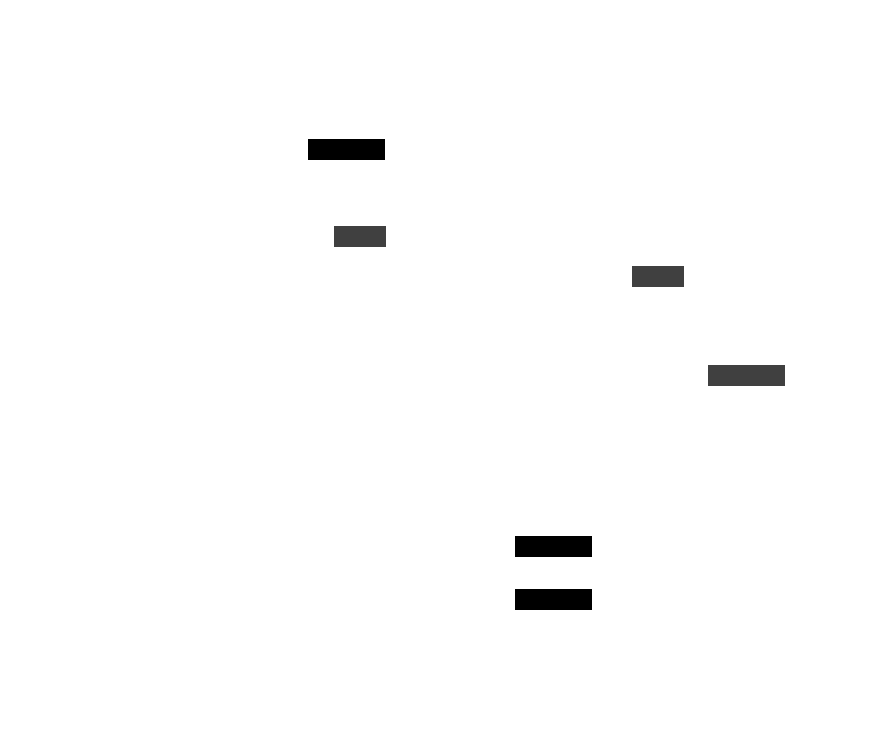
\includegraphics[width=.8\linewidth]{diagram/pipeline.png}
            \caption{Global processing pipeline for the study}
            \label{fig:pipeline}
        \end{figure}

        Even though the above figure~\ref{fig:pipeline} explicit the global process of this study, it is important to understand that it is flexible and subject to changes. In section~\ref{results}, we will explicit each processing step for all presented models. 

    
\section{Results}\label{results}
    Lorem Ipsum

    \subsection{Empty B}
        Lorem Ipsum

        \subsubsection{Résultats et discussions}
            Lorem Ipsum

            Lorem Ipsum Lorem Ipsum Lorem Ipsum Lorem Ipsum
            Lorem Ipsum Lorem Ipsum Lorem Ipsum Lorem Ipsum
            Lorem Ipsum Lorem Ipsum Lorem Ipsum Lorem Ipsum
            Lorem Ipsum Lorem Ipsum Lorem Ipsum Lorem Ipsum
            Lorem Ipsum Lorem Ipsum Lorem Ipsum Lorem Ipsum
            Lorem Ipsum Lorem Ipsum Lorem Ipsum Lorem Ipsum
            Lorem Ipsum Lorem Ipsum Lorem Ipsum Lorem Ipsum
            Lorem Ipsum Lorem Ipsum Lorem Ipsum Lorem Ipsum
            Lorem Ipsum Lorem Ipsum Lorem Ipsum Lorem Ipsum
            Lorem Ipsum Lorem Ipsum Lorem Ipsum Lorem Ipsum
            Lorem Ipsum Lorem Ipsum Lorem Ipsum Lorem Ipsum
            Lorem Ipsum Lorem Ipsum Lorem Ipsum Lorem Ipsum
            Lorem Ipsum Lorem Ipsum Lorem Ipsum Lorem Ipsum

        %%%%%% ------------------------------------------------------------------- %%%%%



\section*{Conclusion and Perspectives}

In this work, we cite.

\section*{Author's contributions}

\acknow{None}
\showacknow{} % Display the acknowledgments section

\bibliography{references}


\end{document}